% ***********************************************************
% ******************* PHYSICS HEADER ************************
% ***********************************************************
% Version 2.Nacho.1
\documentclass[11pt]{article} 
\usepackage{amsmath} % AMS Math Package
\usepackage{amsthm} % Theorem Formatting
\usepackage{amssymb}	% Math symbols such as \mathbb
\usepackage{graphicx} % Allows for eps images
\usepackage{multicol} % Allows for multiple columns
\usepackage[dvips,letterpaper,margin=0.75in,bottom=0.5in]{geometry}
 % Sets margins and page size
\makeatletter % Need for anything that contains an @ command 
\renewcommand{\maketitle} % Redefine maketitle to conserve space
{ \begingroup \vskip 10pt \begin{center} \large {\bf \@title}
	\vskip 10pt \large \@author \hskip 20pt \@date \end{center}
  \vskip 10pt \endgroup \setcounter{footnote}{0} }
\makeatother % End of region containing @ commands
\renewcommand{\labelenumi}{(\alph{enumi})} % Use letters for enumerate
% \DeclareMathOperator{\Sample}{Sample}
\let\vaccent=\v % rename builtin command \v{} to \vaccent{}
\renewcommand{\v}[1]{\ensuremath{\mathbf{#1}}} % for vectors
\newcommand{\gv}[1]{\ensuremath{\mbox{\boldmath$ #1 $}}} 
% for vectors of Greek letters
\newcommand{\uv}[1]{\ensuremath{\mathbf{\hat{#1}}}} % for unit vector
\newcommand{\abs}[1]{\left| #1 \right|} % for absolute value
\newcommand{\avg}[1]{\left< #1 \right>} % for average
\let\underdot=\d % rename builtin command \d{} to \underdot{}
\newcommand{\der}[2]{\frac{d #1}{d #2}} % for derivatives
\newcommand{\dder}[2]{\frac{d^2 #1}{d #2^2}} % for double derivatives
\newcommand{\dnder}[3]{\frac{d^{#3} #1}{d #2^{#3}}} % para derivadas n-esimas
\newcommand{\dpar}[2]{\frac{\partial #1}{\partial #2}}
\newcommand{\ddpar}[2]{\frac{\partial^2 #1}{\partial #2^2}} % for double partial derivatives
\newcommand{\dnpar}[3]{\frac{\partial^{#3} #1}{\partial #2^{#3}}}% para derivadas parciales n-esimas
\newcommand{\dparc}[3]{\left( \frac{\partial #1}{\partial #2}
 \right)_{#3}} % for thermodynamic partial derivatives
\newcommand{\ket}[1]{\left| #1 \right>} % for Dirac bras
\newcommand{\bra}[1]{\left< #1 \right|} % for Dirac kets
\newcommand{\braket}[2]{\left< #1 \vphantom{#2} \right|
 \left. #2 \vphantom{#1} \right>} % for Dirac brackets
\newcommand{\matrixel}[3]{\left< #1 \vphantom{#2#3} \right|
 #2 \left| #3 \vphantom{#1#2} \right>} % for Dirac matrix elements
\newcommand{\grad}[1]{\gv{\nabla} #1} % for gradient
\let\divsymb=\div % rename builtin command \div to \divsymb
\renewcommand{\div}[1]{\gv{\nabla} \cdot #1} % for divergence
\newcommand{\curl}[1]{\gv{\nabla} \times #1} % for curl
\newcommand{\ssum}[2]{\sum_{#1}^{#2}}
\newcommand{\pprod}[2]{\prod_{#1}^{#2}}
\let\baraccent=\= % rename builtin command \= to \baraccent
\renewcommand{\=}[1]{\stackrel{#1}{=}} % for putting numbers above =
\newtheorem{prop}{Proposition}
\newtheorem{thm}{Theorem}[section]
\newtheorem{lem}[thm]{Lemma}
\theoremstyle{definition}
\newtheorem{dfn}{Definition}
\theoremstyle{remark}
\newtheorem*{rmk}{Remark}

% ***********************************************************
% ********************** END HEADER *************************
% ***********************************************************


\begin{document}
\begin{titlepage}
\newcommand{\HRule}{\rule{\linewidth}{0.5mm}}
\center 
 
\textsc{\LARGE UNIVERSIDAD NACIONAL AUT\'ONOMA DE M\'EXICO}\\[1.5cm] 
\textsc{\Large Facultad de Ciencias}\\[0.5cm] 
\textsc{\large Laboratorio de electr\'onica}\\[0.5cm] 
\HRule \\[0.4cm]
{ \huge \bfseries Pr\'actica III: Fuentes de voltaje}\\[0.4cm]
\HRule \\[1.5cm]
\begin{minipage}{0.4\textwidth}
\begin{flushleft} \large
\emph{Alumno:}\\
Ignacio \textsc{Loaiza}
\end{flushleft}
\end{minipage}
~
\begin{minipage}{0.4\textwidth}
\begin{flushright} \large
\emph{Profesor} \\
Dr. Jos\'e\ Manuel \textsc{Alvarado Reyes}
\end{flushright}
\end{minipage}\\[3cm]
{\large 18 de Septiembre de 2014}\\[0.5cm]
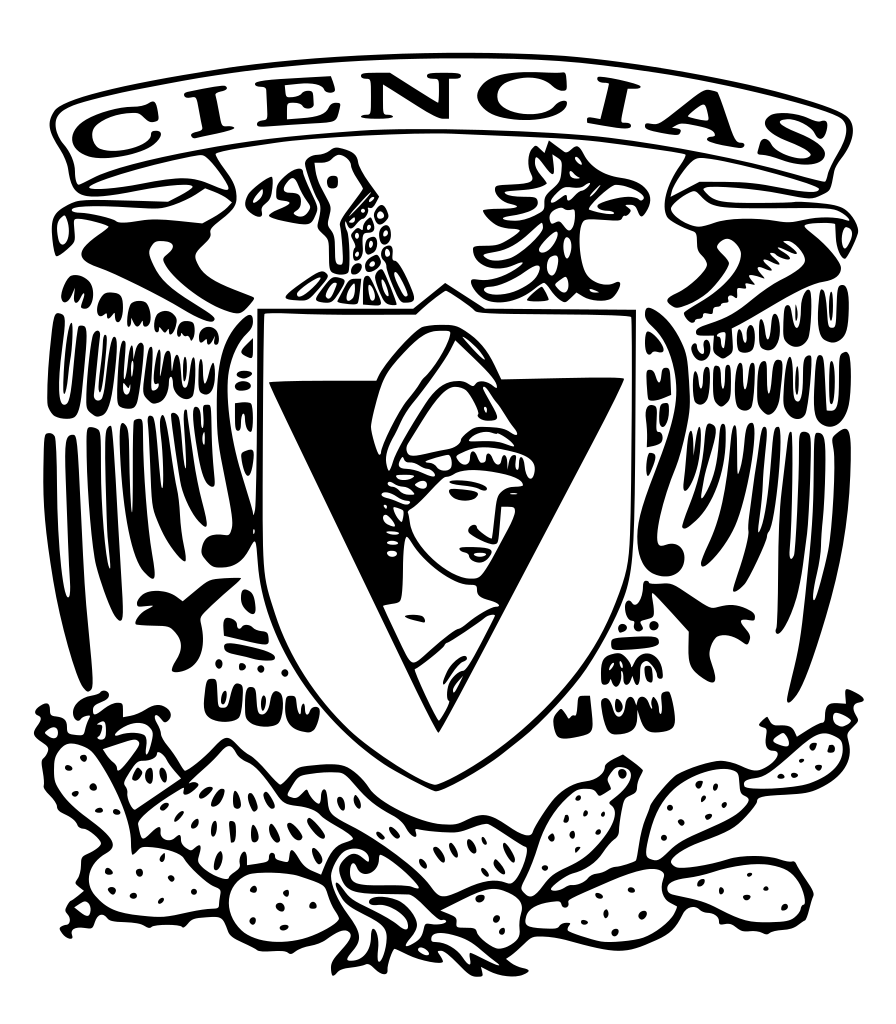
\includegraphics[width=6cm]{/home/nacho/Escuela/ciencias.png}\\[1cm]
\vfill
\end{titlepage}
\section{Resumen}
En esta pr\'actica se fabricaron varias fuentes de voltaje continuo a partir de la toma de corriente. Para hacer esto, primero se estudi\'o\ el comportamiento de los capacitores, los cuales son un componente clave en no s\'olo las fuentes de DC, sino toda la electr\'onica en general. Primero se hizo una fuente de DC simple (sea con dos salidas, una neutra y otra positiva), y luego una fuente doble de DC (con tres salidas: una negativa, una neutra y una positiva). Adem\'as se estudiaron los ruidos que pueden aparecer en estas fuentes, as\'i\ como la forma de minimizarlos.

\section{Introducci\'on}
A lo largo de la carrera se han utilizado un gran n\'umero de veces las fuentes de voltaje continuo, sin realmente saber c\'omo funcionan. Se han estado utilizando como una caja negra, la cual se conecta a la toma de corriente y convierte a la corriente AC en DC. Resulta natural, como prospectos cient\'ificos, estudiar el funcionamiento de estos aparatos.Adem\'as se buscaron maneras para perfeccionar las fuentes y minimizar los errores, lo cual puede ser muy \'util el d\'ia de ma\~nana que haya que utilizar la electr\'onica para alg\'un experimento de investigaci\'on.

\section{Marco te\'orico}
\subsection{Capacitores}
Un capacitor es un elemento que est\'a\ formado de dos placas conductoras separadas por un diel\'ectrico. Los capacitores resultan muy interesantes ya que son capaces de almacenar un voltaje, y luego pueden actuar, durante un corto periodo de tiempo, como una fuente de voltaje. En este reporte no se van a deducir las ecuaciones de carga y descarga de un capacitor, tan s\'olo se van a citar. \\
Si se tiene un capacitor conectado en un circuito como el que se ve a continuaci\'on:
\begin{center}
\includegraphics[width=10cm]{capa.png}
\end{center}
\begin{center}
Esquema 1: Circuito de carga y descarga del capacitor.
\end{center}
En este circuito, la resistencia $R1$ corresponde a la de la carga, y $R2$ a la de descarga. Se puede controlar en qu\'e\ r\'egimen est\'a\ el sistema con los interruptores $S1$ (para la carga) y $S2$ (para la descarga). El tiempo de carga o de descarga est\'a\ dado por la siguiente ecuaci\'on:
\begin{equation}
\tau=RC
\end{equation}
Con $R$ la resistencia en Ohms $[\Omega]$ (de carga o de descarga), y $C$ la capacitancia en Farads $[F]$.
En la fase de carga, el voltaje de un capacitor sigue la siguiente ecuaci\'on:
\begin{equation}
V_c=V(1-e^{\frac{-t}{\tau_c}})=V(1-e^{\frac{-t}{R1*C}})
\end{equation}
Y en la fase de descarga es:
\begin{equation}
V_d=Ve^{\frac{-t}{\tau_d}}=Ve^{\frac{-t}{R2*C}}
\end{equation}
Adem\'as, la reactancia capacitiva est\'a\ dada por:
\begin{equation}
X_c=\frac{1}{\omega C}=\frac{1}{2\pi fC}
\end{equation}
La reactancia capacitiva est\'a\ relacionada con la impedancia de un circuito, e indica cuanta resistencia ofrece un circuito al paso de la corriente. La inductancia se mide en Ohms $[\Omega]$, tiene una magnitud y una fase (la fase s\'olo aparece en corrientes alternas) y est\'a\ dada por:
\begin{equation}
Z=R+jX
\end{equation}
D\'onde $R$ es la resistencia del circuito, $X$ es la reactancia (y es la fase de la impedancia), y $j$ es el valor imaginario que corresponde a $j^2=-1$.
\section{Experimentaci\'on}
\subsection{Capacitores}
\subsubsection{Materiales}
\begin{itemize}
\item Resistencia de $5$ $K\Omega$
\item Capacitor de $1000 \mu F$
\item Fuente simple de DC
\item Osciloscopio
\end{itemize}
\subsubsection{M\'etodo experimental}
Se conect\'o\ el capacitor primero a un circuito de carga con un voltaje de le fuente de $10V$ (corriente cont\'inua), y se observ\'o\ el voltaje del capacitor en el osciloscopio. Luego se conect\'o\ el capacitor en el ciclo de descarga, y se observ\'o\ su voltaje en el osciloscopio.

\subsubsection{Resultados y discusi\'on}
Antes que nada, cabe notar que esta pr\'actica nada m\'as se hizo con el fin de verificar el comportamiento de un capacitor, y no se consider\'o\ necesario repetir el experimento con valores distintos de los componentes. \\
En el ciclo de carga y de descarga, se obtuvo un tiempo de carga (aproximadamente) de 5 segundos. (El tiempo de carga est\'a\ definido por el tiempo que le toma al capacitor cargarse al $63.2\% $ del voltaje suministrado, o de descargarse al $36.8\% $ de su voltaje inicial. El c\'alculo te\'orico del tiempo de carga/descarga da $\tau=R*C=5*10^3*1*10^{-3}=	5s$. Se obtuvieron gr\'aficas para la carga y descarga de acuerdo con las gr\'aficas te\'oricas (que siguen el comportamiento de las ecuaciones $(2)$ y $(3)$). Se logr\'o\ confirmar entonces el comportamiento de los capacitores, lo cual permitir\'a\ m\'as adelante hacer la selecci\'on correcta de un capacitor para el circuito a armar.

\subsection{Fuente simple}
\subsubsection{Materiales}
\begin{itemize}
\item Transformador de $12V_{rms}$
\item Diodos
\item Capacitores de $100$, $850$, $1000$ y $5600$ $\mu F$
\item Transistor 7805
\item Osciloscopio
\item Resistencia de $1k\Omega$.
\item Resistencias de potencia de baja resistencia
\end{itemize}
\subsubsection{M\'etodo experimental}
Para armar la fuente simple, se tomaron varios pasos, y en cada uno se cambiaron algunas cosas, de forma que se entendiera qu\'e\ estaba haciendo qu\'e\ componente y porqu\'e\. Sin embargo, en general se busc\'o\ llegar a una fuente como la que se ve a continuaci\'on:
\begin{center}
\includegraphics[width=10cm]{simple.png}
\end{center}
\begin{center}
Esquema 2: Circuito correspondiente a una fuente simple de DC. 
\end{center}
Cabe notar que, para las mediciones de los voltajes de salida (los cuales se mideiron en el osciloscopio), hubo que poner una resistencia en la salida, ya que de otra forma no se generaba ninguna corriente y las mediciones eran inservibles.
\subsubsection*{El transformador con el puente de diodos}
Se coloc\'o\ al transformador a la salida de la toma de corriente. Luego, a la salida del transformador, se utilizaron dos m\'etodos distintos: el de media onda y el de onda completa, como se ve en los esquemas a continuaci\'on:
\begin{center}
\includegraphics[width=10cm]{ondacomp.png}
\end{center}
\begin{center}
Esquema 3: Salida de onda completa.
\end{center}
Y:
\vspace{5cm}
\begin{center}
Esquema 4: Salida de media onda.
\end{center}
\subsubsection*{Capacitor y voltaje Rizo}
Luego, se le a\~nadi\'o\ un capacitor a la salida como se ve a continuaci\'on:
\begin{center}
\includegraphics[width=10cm]{tocapa.png}
\end{center}
\begin{center}
Esquema 5: Circuito con transformador, rectificador y capacitor.
\end{center}
Se cambi\'o\ este capacitor de forma que se observ\'o\ el comportamiento de la salida dependiendo del capacitor aqu\'i\ colocado, midiendo los cambios en el voltaje Rizo.

\subsubsection*{Transistor}
Despu\'es se le coloc\'o\ el transistor al circuito (sea el regulador) y se volvi\'o\ a medir el voltaje de salida.

\subsubsection*{Capacitor salida}
Finalmente se le coloc\'o\ el otro capacitor a la salida, obteniendo la funete simple como se puede ver en el esquema (2), y se volvi\'o\ a medir el voltaje.

\subsubsection*{Impedancia}
Se busc\'o\ medir la impedancia de la fuente creada. Para hacer esto, se estudi\'o\ el voltaje de salida
\subsubsection{Resultados y discusi\'on}
Antes que nada cabe notar que el voltaje pico a la salida del transformador fue de $20V$, con una frecuencia de $60.24Hz$.
\subsubsection*{Transformador y puente de diodos}
El puente de diodos volvi\'o\ positivo al voltaje, s\'olo dejando pasar a la norma de este, como era de esperarse sabiendo que los diodos s\'olo permiten pasar a la corriente en un sentido. Cuando se tom\'o\ la salida de onda completa, se obtuvo un voltaje con $V_p=20V$, con una frecuencia de $120.48Hz$:
\begin{center}
\includegraphics[width=6cm]{recti.png}
\end{center} 
\begin{center}
Gr\'afica 6: Representaci\'on cualitativa del voltaje de salida de onda completa.
\end{center}
Este comportamiento se obtuvo entonces al rectificar (sea tomar la norma) de un voltaje sinusoidal con mismo valor de voltaje pico. \\
Al tomarla salida de media onda, se obtuvo un voltaje pico de $20V$ con una frecuencia de $60.24Hz$, con un comportamiento de la forma siguiente:
\begin{center}
\includegraphics[width=8cm]{media.png}
\end{center} 
\begin{center}
Gr\'afica 7: Representaci\'on cualitativa del voltaje de salida de media onda.
\end{center}
Este comportamiento se debe a que, al tomar una de las salidas del transformador como la tierra, al medir el voltaje con respecto a esta tierra s\'olo hay una de las dos secciones del voltaje inicial que "sobrevive", teniendo que esta parte del voltaje es la que se ve en la salida.

\subsubsection*{Capacitor y voltaje Rizo}
Al colocar un capacitor a la salida, se obtuvo un voltaje como se ve a continuaci\'on:
\begin{center}
\includegraphics[width=8cm]{media.png}
\end{center} 
\begin{center}
Gr\'afica 8: Voltaje cont\'inuo con voltaje Rizo.
\end{center}
Se obtuvo un voltaje cont\'inuo de $18V$ con voltajes Rizo que var\'ian como se ve en la tabla (1) en funci\'on del capacitor utilizado.
\begin{center}
\begin{tabular}{||c|c||}
\hline
Valor del capacitor $[\mu F]$ & Voltaje Rizo pico pico $[V_{pp}]$ \\ \hline
100 & 2 \\ \hline
850 & 1 \\ \hline
1000 & 0.12 \\ \hline
5600 & 0.13 \\ \hline
\end{tabular}
\end{center}
\begin{center}
Tabla 1: Valores del votlaje Rizo pico pico en funci\'on del capacitor utilizado.
\end{center}
Cabe notar que las frecuencias del voltaje Rizo en todos los casos fue de $121Hz$. Este comportamiento se debe a que, con voltajes AC cont\'inuos, el ciclo de carga y descarga del capacitor se ve como la figura a continuaci'on (la resistencia es casi nula en la carga, teniendo que se carga de forma pr\'acticamente instant\'anea, mientras que en la descarga la resistencia es la resistencia de salida de carga, teniendo un tiempo m\'as significativo).
\begin{center}
\includegraphics[width=8cm]{rizo.png}
\end{center} 
\begin{center}
Gr\'afica 9: Explicaci\'on del voltaje Rizo.
\end{center}
Al tener capacitores con una gran capacitancia, el tiempo de descarga disminuye dr\'asticamente, causando entonces esa disminuci\'on en el voltaje Rizo.

\subsubsection*{Transistor}
El transistor (o regulador) es un elemento cuyo funcionamiento interno no se estudi\'o\ en esta pr\'acitca. Al colocar el transistor, el voltaje de salida se volvi\'o\ de $5V$ cont\'inuos, con un ruido de $6mV$ pico a una frecuencia de $121Hz$. Se puede ver c\'omo este elemento termin\'o\ de transformar al voltaje alterno en voltaje continuo, eliminando casi por completo al voltaje Rizo.

\subsubsection*{Capacitor salida}
Finalmente, al colocar el capacitor a la salida (se utiliz\'o\ el de $5600\mu F$), no se alcanz\'o\ a medir ninguna mejora en cuanto a una disminuci\'on en el ruido del voltaje. Sin embargo, el ruido era tan peque\~no para comenzar que la medici\'on correcta es dif\'icil con la instrumentaci\'on utilizada.

\subsubsection*{Impedancia}
El primer transformador utilizado ten\'ia un l\'imite de corriente de $300mA$, los cuales eran utilizados al colocar una resistencia a la salida de $18\Omega$. El voltaje de salida no sufri\'o\ de ninguna ca\'ida con esta resistencia, y ya no se quiso disminuir m\'as la resistencia por miedo a da\~nar el transformador. Se cambi\'o\ entonces el transformador a uno con un voltaje de salida un poco m\'as bajo (aunque el voltaje obtenido a la salida de la fuente fue el mismo). Este segundo transformador ten\'ia una corriente m\'axima de $3A$, pudiendo alimentar a una resistencia de hasta $2\Omega$ sin riesgo a quemarlo. Para las resistencias mayores a $15\Omega$ el voltaje de salida sali\'o\ sin ser modificado. Para resistencias entre $2\Omega$ y $10\Omega$, la fuente sigue funcionando, aunque el regulador (transistor) ya no funciona correctamente. Sin embargo se logr\'o\ concluir que la impedancia de la fuente fabricada es menor a $2\Omega$.

\subsection{Fuente doble}
\subsubsection{Materiales}
\begin{itemize}
\item Transformador
\item Puente de diodos
\item Capacitores de $1000\mu F$
\item Transistores 7812 y 7912.
\end{itemize}
\subsubsection{M\'etodo experimental}
Se arm\'o\ la fuente doble como el circuito siguiente:
\begin{center}
\includegraphics[width=10cm]{doble.png}
\end{center} 
\begin{center}
Esquema 10: Fuente de voltaje doble.
\end{center}
Se midi\'o\ el voltaje en las diferentes salidas de la fuente.

\subsubsection{Resultados y discusi\'on de la fuente doble}
Al medir el voltaje, se obtuvo que entre cada salida hab\'ia una diferencia de $12V_{DC}$, teniendo que entre la salida negastiva y la positiva hubo una diferencia de $24V$. El voltaje Rizo medido gue de $20mV_{pp}$, con una frecuencia de $121Hz$. Esta fuente se hizo entonces para verificar que se entendi\'o\ el funcionamiento de los componentes de una fuente de voltaje continuo.


\section{Conclusi\'on}
Se observ\'o\ y comprendi\'o\ satisfactoriamente el funcionamiento de un capacitor. A partir de este conocimiento, se logr\'o\ fabricar una fuente de corriente continua simple y una doble, entendiendo para que sirve cada componente, de forma que ya se sabe que hay adentro de la "caja negra" que se utiliza por lo general. Cabe notar que, al disminuir la cantidad de elementos que se tiene en la fuente, la impedancia de esta disminuye, por lo cual, al fabricar una fuente, hay que tomar en cuenta este factor y llegar a un buen balance entre precisi\'on (con poco ruido, voltaje Rizo bajo) y practicidad (impedancia baja para poder hacer m\'as experimentos). 

\section{Bibliograf\'ia}
\begin{enumerate}
\item I. Loaiza, \textit{Bit\'acora de laboratorio de electr\'onica 2015-1}.
\end{enumerate}
\end{document}
